\documentclass{article}
\usepackage{graphicx} % Required for inserting images
\usepackage{amsmath}
\usepackage{algorithm}
\usepackage{algpseudocodex}
\usepackage{float}
\usepackage{placeins}
\usepackage{etoolbox}
\usepackage{amssymb}
\usepackage{hyperref}
\usepackage{booktabs}
\usepackage{xcolor}
\usepackage{tikz}
   \usetikzlibrary{positioning}
\usepackage{pgfplots}
\usepgfplotslibrary{groupplots}
\usepgfplotslibrary{statistics}
   \pgfplotsset{compat=1.18}
%%PREAMBLE%%
\usepackage{pdflscape}
\usepackage[margin=1in]{geometry}
% Tall result figures: prefer top-of-page placement with following text
% underneath, instead of a vertically centered float-only page.
\renewcommand{\topfraction}{0.95}
\renewcommand{\textfraction}{0.05}
\renewcommand{\floatpagefraction}{0.8}
\makeatletter
\setlength{\@fptop}{0pt}
\setlength{\@fpbot}{0pt plus 1fil}
\makeatother
% Wide appendix tables: landscape PDF pages via pdflscape.
\newenvironment{landscapetable}{%
 \clearpage
 \begin{landscape}%
}{%
 \end{landscape}%
 \clearpage
}


\title{A Novel Application of Ant Colony Optimization to $k$-defective Maximum Edge Bicliques}
\author{Kiyaan Pillai}
\date{September 2026}


%     Custom "parallel for each" block, wired into algpseudocodex's
%     internal indent/highlight hooks (bare \algdef breaks the package's
%     block tra cking and throws \endcsname errors)
\makeatletter
\algdef{SE}[FORPAR]{ForPar}{EndForPar}[1]%
 {\algpx@startIndent\algpx@startCodeCommand\textbf{parallel for each}\ #1\ \algorithmicdo}%
 {\algpx@endIndent\algpx@startCodeCommand\algorithmicend\ \textbf{parallel for each}}%


\ifbool{algpx@noEnd}{%
 \algtext*{EndForPar}%
 \apptocmd{\EndForPar}{\algpx@endIndent}{}{}%
}{}%


\pretocmd{\ForPar}{\algpx@endCodeCommand}{}{}
\ifbool{algpx@noEnd}{%
 \pretocmd{\EndForPar}{\algpx@endCodeCommand[1]}{}{}%
}{%
 \pretocmd{\EndForPar}{\algpx@endCodeCommand[0]}{}{}%
}%
\makeatother


\begin{document}
\maketitle


\begin{abstract}
The maximum $k$-defective edge biclique ($k$-MDB) problem is an emerging NP-hard optimization. We adapt Ant Colony Optimization (ACO) to the k-MDB problem, introducing a local neighborhood search to improve solution quality. In many instances, ACO produces bicliques with $80\%$ or more edges than previously proposed heuristics. Additionally, ACO provides a tighter lower bound on the size of the $k$-MDB and can cut brute force search time by more than half.
\end{abstract}


\section{Introduction}


A bipartite graph is a common graph structure where one set of vertices is connected solely to another. Bipartite graphs can model user-product behavior, person-place interaction, and more. A biclique is a set of vertices on a bipartite graph such that each vertex on one side is connected to each vertex on the other. The maximum edge biclique problem aims to identify the biclique with the most edges on a bipartite graph. The problem has applications in online recommendation systems, fraud detection, and community detection [1].


One example of bicliques' utility is in e-commerce fraud detection, where a bipartite graph could represent users and the products they buy. A set of accounts that purchase overlapping sets of items may represent a coordinated fraud ring, yielding a subgraph that is almost fully connected across the two sides. Requiring a perfect biclique would discard this signal whenever a few transactions are omitted deliberately or lost to incomplete logging. A dense, near-biclique structure remains interpretable under small amounts of noise; perfect completeness does not matter.


Generally, real-world data often introduces noise to graphs, and structures with relatively few missing connections may still be relevant. A biclique that is allowed up to $k$ missing edges, or a $k$-defective biclique ($k$-DB), can overcome this real-world noise. Identifying the maximum $k$-defective edge biclique ($k$-MDB) remains an emerging field.


\begin{figure}[H]
   \centering
   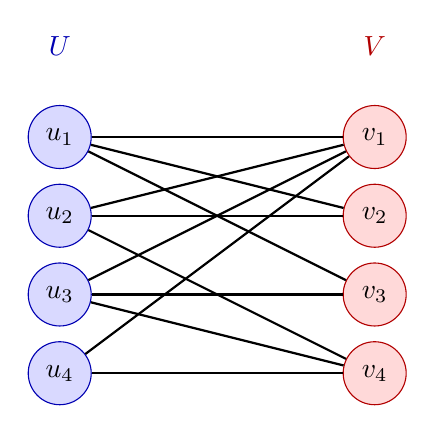
\begin{tikzpicture}[
       Uvertex/.style={
           circle,
           draw=blue!70!black,
           fill=blue!15,
           minimum size=8mm
       },
       Vvertex/.style={
           circle,
           draw=red!70!black,
           fill=red!15,
           minimum size=8mm
       },
       edge/.style={thick}
   ]


   % Left side U
   \node[Uvertex] (u1) at (0,2) {$u_1$};
   \node[Uvertex] (u2) at (0,1) {$u_2$};
   \node[Uvertex] (u3) at (0,0) {$u_3$};
   \node[Uvertex] (u4) at (0,-1) {$u_4$};


   % Right side V
   \node[Vvertex] (v1) at (4,2) {$v_1$};
   \node[Vvertex] (v2) at (4,1) {$v_2$};
   \node[Vvertex] (v3) at (4,0) {$v_3$};
   \node[Vvertex] (v4) at (4,-1) {$v_4$};


   % Edges
   \draw[edge] (u1) -- (v1);
   \draw[edge] (u1) -- (v2);
   \draw[edge] (u1) -- (v3);


   \draw[edge] (u2) -- (v1);
   \draw[edge] (u2) -- (v2);
   \draw[edge] (u2) -- (v4);


   \draw[edge] (u3) -- (v1);
   \draw[edge] (u3) -- (v3);
   \draw[edge] (u3) -- (v4);


   \draw[edge] (u4) -- (v1);
   \draw[edge] (u4) -- (v4);


   % Labels
   \node[above=5mm of u1] {\textcolor{blue!70!black}{$U$}};
   \node[above=5mm of v1] {\textcolor{red!70!black}{$V$}};


   \end{tikzpicture}
   \caption{Example bipartite graph $G=(U,V,E)$}
   \label{fig:bipartite-example}
\end{figure}


\begin{figure}[H]
   \centering
   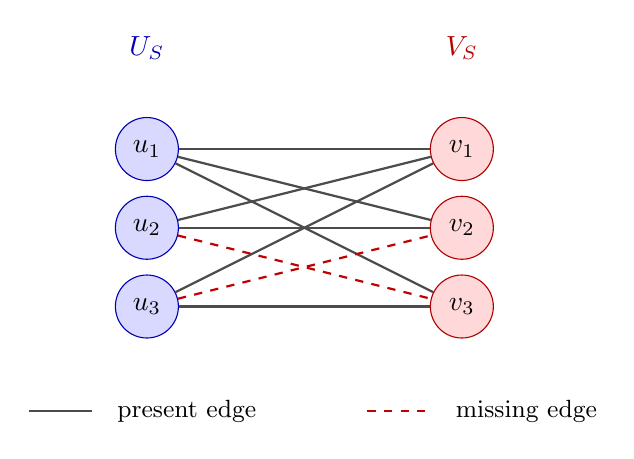
\begin{tikzpicture}[
       Uvertex/.style={
           circle,
           draw=blue!70!black,
           fill=blue!15,
           minimum size=8mm
       },
       Vvertex/.style={
           circle,
           draw=red!70!black,
           fill=red!15,
           minimum size=8mm
       },
       edge/.style={
           thick,
           draw=black!70
       },
       missing/.style={
           thick,
           dashed,
           draw=red!75!black
       }
   ]


   % Vertices
   \node[Uvertex] (u1) at (0,2) {$u_1$};
   \node[Uvertex] (u2) at (0,1) {$u_2$};
   \node[Uvertex] (u3) at (0,0) {$u_3$};


   \node[Vvertex] (v1) at (4,2) {$v_1$};
   \node[Vvertex] (v2) at (4,1) {$v_2$};
   \node[Vvertex] (v3) at (4,0) {$v_3$};


   % Present edges
   \draw[edge] (u1) -- (v1);
   \draw[edge] (u1) -- (v2);
   \draw[edge] (u1) -- (v3);


   \draw[edge] (u2) -- (v1);
   \draw[edge] (u2) -- (v2);


   \draw[edge] (u3) -- (v1);
   \draw[edge] (u3) -- (v3);


   % Missing edges
   \draw[missing] (u2) -- (v3);
   \draw[missing] (u3) -- (v2);


   % Set labels
   \node[above=6mm of u1]
       {\textcolor{blue!70!black}{$U_S$}};
   \node[above=6mm of v1]
       {\textcolor{red!70!black}{$V_S$}};


   % Centered legend
   \node[below=12mm of $(u3)!0.5!(v3)$] (legend) {};


   \draw[edge]
       ([xshift=-35mm]legend.center) --
       ([xshift=-27mm]legend.center);
   \node[anchor=west, font=\small]
       at ([xshift=-25mm]legend.center) {present edge};


   \draw[missing]
       ([xshift=8mm]legend.center) --
       ([xshift=16mm]legend.center);
   \node[anchor=west, font=\small]
       at ([xshift=18mm]legend.center) {missing edge};


   \end{tikzpicture}


   \caption{
       A $2$-defective biclique present in Figure~\ref{fig:bipartite-example}. Every vertex in $U_S$ is connected
       to every vertex in $V_S$ except for two missing edges.
       Since $|\bar{E}(S)|=2$, this is a $2$-defective biclique. In fact, it is a $k$-defective biclique for any $k \geq 2$.
   }
   \label{fig:k-defective-biclique}
\end{figure}


Maximizing edge count alone is not enough for real-world interpretability. Without a lower bound on each side's size, the optimum is often a lopsided subgraph with many edges but little practical significance. In the case of fraud, a single popular item purchased by thousands of unrelated users could be a massive biclique with one vertex opposite many others, but it signals mass-market demand rather than a coordinated ring. We therefore seek only $\theta$-feasible \mbox{$k$-DB}: \mbox{$k$-DB} where both sides have at least $\theta$ vertices, where $\theta$ is a user-defined parameter.


The $k$-MDB problem is NP-hard. Unless P = NP, there is no algorithm that can run in polynomial time and is guaranteed to find the maximum solution. When the absolute optimum is not necessary, approximation techniques are useful to significantly reduce computation while providing meaningfully large bicliques. The only heuristic in literature for this problem is proposed by Cui et al., referred to in this paper as the $\theta$-heuristic. Cui et al. also propose a brute-force algorithm to find the $k$-MDB called branch-and-pivot.


Dorigo et al. [2] proposed a metaheuristic known as Ant Colony Optimization (ACO) for exploring graphs. Initially used on finding the shortest path in the Traveling Salesman Problem, ACO has been adapted to many graph problems, such as vehicle routing [5], quadratic assignment [6], graph coloring [7], and the maximum clique problem [8].


We introduce an ACO-inspired heuristic for the $k$-defective maximum edge biclique ($k$-MDB) problem, incorporating a neighbor-scope restriction that reduces the set of vertices considered during construction. Across 37 benchmark graphs, ACO frequently finds larger and more often $\theta$-feasible solutions than the existing $\theta$-heuristic, although at substantially higher computational cost. We further show that these stronger solutions can improve branch-and-pivot search, reducing its wall-clock time by up to $56\%$ on tested instances. Together, these results demonstrate ACO as a complementary approach to existing $k$-MDB heuristics, trading increased search cost for improved solution quality.


\section{Background}


\subsection{Definitions}


Define a bipartite graph as a graph $G = (U, V, E)$, where $U$ and $V$ are two disjoint sets of vertices, and $E \subseteq U \times V$ is the set of edges between $U$ and $V$. Let $S = (U_S, V_S)$ denote a set of vertices where $U_S \subseteq U$ and $V_S \subseteq V$. Let $E_S = \{(u, v) \mid u \in U_S \wedge v \in V_S \wedge (u, v) \in E \}$ be the set of edges in a subgraph $S$. Define $\bar{E}(S) = \{(u, v) \mid u \in U_S \wedge v \in V_S \wedge (u, v) \not\in E \}$ be the set of non-edges in a subgraph. Let a $k$-defective biclique be a subgraph $S$ where $|\bar{E}(S)| \leq k$. Because every possible edge runs between the two sides of a biclique, a subgraph with $|U_S|$ and $|V_S|$ vertices has at most $|U_S||V_S|$ edges. For a $k$-defective biclique, $|E(S)|=|U_S||V_S|-|\bar E(S)|$, with $|\bar E(S)|\le k$.


Define the neighbors of a vertex $u$ in a subgraph $S$ as $N_S(u) = \{v \in S \mid \{u, v\} \in E(S)\}$. Define the nonneighbors of a vertex as $\bar{N}_S(u) = \{v \in S \mid (u, v) \not\in E(S)\}$. Define the degree of a vertex as $d_S(u) = |N_S(u)|$, and the nondegree as $\bar{d}_S(u) = |\bar{N}_S(u)|$.


Define the maximum $k$-MDB as the $k$-DB with the largest number of edges in a graph $G$. Let $\theta$ be a user-defined minimum side size. The algorithms proposed in this paper seek the maximum $k$-MDB $D^*$ with $|U_{D^*}| \geq \theta$ and $|V_{D^*}| \geq \theta$ as described in Section~1. We require that $\theta > k$. A vertex on one side can have at most $|V_S|$ missing edges. If $|V_S| \le k$, then even a vertex with zero neighbors can satisfy the $k$-defective constraint. Therefore requiring $\theta>k$ ensures every vertex in a $\theta$-feasible $k$-DB must have at least one neighbor.


\subsection{Computational Complexity}


Finding the maximum $k$-MDB on a bipartite graph is an NP-hard optimization problem. The maximum clique problem reduces to the $k$-MDB problem [1]. Because the maximum clique is NP-hard, the $k$-MDB problem is NP-hard as well.


\subsection{Previous Work}


Similar dense subgraph models provide precedent for the $k$-MDB. In non-partite graphs, \emph{defective cliques}, cliques that are missing up to a certain number of edges, have been used to recover nearly complete structures from noisy biological interaction graphs [12]. On bipartite graphs, relaxed models include $k$-biplexes, which permit each vertex up to $k$ nonneighbors in the biplex [15], and $k$-defective bicliques, which have a tighter restriction of only allowing up to $k$ total missing edges. The $k$-MDB generalizes to the maximum edge biclique when $k = 0$ [1], [11].


Cui et al. [1] proposed a brute-force approach to the $k$-MDB problem, as well as an initial heuristic designed to find a $k$-MDB with exactly $\theta$ vertices on one side of the graph, described in Section~1. Concurrently, Wang et al. [11] studied the related problem of finding a $k$-defective biclique with the largest vertex count rather than edge count. Because their objective differs from ours, we do not benchmark against their algorithm.


Ant Colony Optimization is a natural metaheuristic for problems where high-quality solutions are built by iteratively adding vertices to a subgraph. In the maximum clique problem, ACO algorithms construct cliques greedily while using pheromone to reinforce vertices that are likely to appear in large solutions [8]. The $k$-MDB problem structure lends itself well to this algorithm: an ant can grow a near-biclique one vertex at a time, checking at each step whether the defect budget permits another addition. These considerations motivate our choice of ACO over alternative metaheuristics for identifying large $k$-DB.


To our knowledge, the $\theta$-heuristic of Cui et al. [1] is the only published heuristic algorithm for the $k$-MDB problem. ACO is therefore compared against the only existing heuristic baseline in the literature.


\section{Methods}


\subsection{ACO Algorithm}


\subsubsection{Overview of Algorithm}


ACO traditionally uses a set of agents, called ``ants'', that traverse a graph and build a solution that must meet certain constraints. The ants leave pheromone on the vertices they visit, attracting other ants to follow their path. As the ants explore the solution space, they all converge on the same vertices as the quantity of pheromones on that path becomes increasingly larger.


We adapt the ACO algorithm to the $k$-MDB problem. A population of ants iteratively adds vertices from $G$ to a subgraph $S$, preferring vertices with higher subgraph degree $d_S$, higher global degree $d_G$, and higher pheromone $\tau$. Across ants and epochs, vertices repeatedly selected in high-quality solutions accumulate pheromone, increasing their likelihood of future selection.


We also add an optional control that improves practical runtime and performance. Flag $F_N$ (neighbor-scope restriction) restricts candidates to the intersection of the $k$-feasible candidate set and the last-added vertex's neighbors when that intersection is nonempty, substantially reducing the set of vertices an ant must score at each step.


As an example, consider an ant has constructed $S$ and its last added vertex is $v_{last}$. If candidates $u_1,u_2,u_3$ preserve the $k$-defect bound but only $u_1,u_2$ are adjacent to $v_{last}$, the neighbor-scope rule restricts the ant to $\{u_1,u_2\}$. It then samples between them according to their pheromone and desirability scores, adds the selected vertex, and repeats until no feasible candidate remains. $F_N$ enables this flag and is our default for all experiments unless noted otherwise.


\subsubsection{Algorithm Pseudocode}


Algorithm~\ref{alg:aco} implements the ant colony loop with optional neighbor-scope restriction~$F_N$. Here, $\sigma(x) = 1/(1+e^{-x})$ denotes the standard logistic sigmoid, used to dampen the impact of a vertex's degree with the entire graph as the size of the subgraph grows. Algorithm~\ref{alg:desirability} implements desirability.


\begin{algorithm}[H]
\caption{ACO}
\label{alg:aco}
\begin{minipage}{\textwidth}
\begin{algorithmic}
   \Require A bipartite graph $G$; hyperparameters $T$, $A$, $F_N$, $\rho$, and $\Delta\tau$; parameters $k$ and $\theta$
   \Ensure a $k$-MDB of $G$, if one could be found
  
  
   \Function{ACO}{$G$, $T$, $A$, $F_N$, $\rho$, $\Delta\tau$}
       \Comment{$F_N$: neighbor-scope flag}
       \ForAll{$u \in G$}
           \State $\tau(u) \gets 1$
       \EndFor   
  
       \State $B \gets \{\}$
  
  
       \For{$e \gets 1,\ldots,T$}
           \State $\mathcal{S} \gets A$ empty subgraphs
           \State $\tau_C \gets \tau$
  
  
           \ForPar{$S_i \in \mathcal{S}$}
               \State $C \gets \{u \in G \mathrel{\text{s.t.}} |\bar{E}(S_i \cup \{u\})| \leq k\}$
               \While{$|C| > 0$}
                   \If{$S_i = \emptyset$}
                       \State $search \gets C$
                   \Else
                       \State $v_{last} \gets$ the last vertex that was appended to $S_i$
                       \State $C_{v_{last}} \gets N(v_{last})$
      
      
                       \If{$|C \cap C_{v_{last}}| > 0$ and $F_N$}
                           \State $search \gets C \cap C_{v_{last}}$
                       \Else
                           \State $search \gets C$
                       \EndIf
                   \EndIf
  
                   \State $next \gets \text{linear sample of } u \in search$ based on  $\Call{desirability}{u, S_i, \tau_C}$
                   \State add $next$ to $S_i$
                   \State $\tau_C(next) \gets \tau_C(next) + \Delta\tau$ \Comment{updates to $\tau_C$ are atomic}


                   \State $C \gets \{u \in G \mid k \geq |\bar{E}(S_i \cup \{u\})|\}$
               \EndWhile
           \EndForPar


           \State $S_B \gets \text{argmax}_{S_i \in \mathcal{S}}{|E(S_i)|}$ \Comment{$S_B$ is guaranteed to have at least one vertex}
  
           \If{$E(S_B) > E(B)$}
               \State $B \gets S_B$
           \EndIf
  
           \State $\tau \gets \tau_C$
  
           \ForAll{$u \in G$}
               \State $\tau(u) \gets \tau(u) \times (1 - \rho)$
           \EndFor
       \EndFor
       \State \Return $B$
   \EndFunction
\end{algorithmic}    
\end{minipage}
\end{algorithm}


We introduce a desirability function that prefers vertices with higher $d_S$, higher $d_G$, and higher pheromone $\tau$.


\begin{algorithm}[H]
\caption{Desirability}
\label{alg:desirability}
\begin{minipage}{\textwidth}
\begin{algorithmic}


\Function{Desirability}{$next, S, \tau$}
   \State $\eta \gets d_S(next) + d_G(next) \times (1 - \sigma(|U_S| + |V_S|))$
   \State \Return $\tau(next) \times \eta^3$
\EndFunction


\end{algorithmic}
\end{minipage}
\end{algorithm}


The $\eta$ exponent was ablated over $\{1, 2, 3\}$, and $3$ demonstrated the best quality.


We also tried elitist pheromone deposition, local tabu search, the MAX-MIN Ant System [4], a genetic algorithm adapted from GCLIQUE [3], and a prefer-smaller-side desirability bias (flag~$F_P$) that multiplies $\eta$ by a constant when exactly one side of the ant's subgraph has reached $\theta$ and the candidate lies on the deficient side. None of the first four outperformed base ACO; the genetic algorithm failed on large graphs, indicating that it struggles with the dimensionality of large bicliques. Alone, $F_P$ improves solution quality over plain ACO, but once neighbor-scope restriction~$F_N$ is enabled it contributes nothing further (Section~4.3).


\subsubsection{Validity Guarantee}


An ant iteratively searches over a set of vertices $C$ such that any vertex $v \in C$ results in $\leq k$ missing edges if added to $S$. Flag~$F_N$ considers the intersection of this set with another. In either case, an ant is guaranteed to only add vertices that adhere to the $k$ constraint. An ant is not guaranteed to return a $k$-DB with $\geq \theta$ vertices on both sides, even on graphs where such a $k$-DB exists, which is a limitation of the $\theta$-heuristic as well. However, we observe that ACO is more likely to return $\theta$-feasible solutions than the $\theta$-heuristic (Section~4.3).


\subsubsection{Theoretical Time Complexity}


Here we analyze the upper complexity bound of our ACO implementation.


\textbf{Subgraph Exploration}
Throughout this analysis, $n = |U| + |V|$ and $m = |E|$ refer to the graph on which ACO runs. In our experiments, ACO runs on graphs that have undergone common-neighbor reduction (Section~3.2), rather than the original graph. For each ant, it must first examine $n$ vertices. At every subsequent step, it will need to consider all vertices it can add to its subgraph without violating the $k$ constraint. A naive approach would examine $n - 1$ vertices, and then $n - 2$ vertices, etc. Thus, an ant will examine at most $n + (n - 1) + (n - 2) \ldots = n(n + 1)/2$.
\


\textbf{Upper Bound} The upper time complexity would therefore be $\mathcal{O}(A \times T \times n^2)$ for $A$ ants advancing over $T$ epochs. In a parallelized implementation with $p$ processors, the true upper complexity bound is $\mathcal{O}(\lceil A / p \rceil \times T \times n^2)$.


\subsubsection{Practical Complexity}


In practice, however, there are two factors limiting this complexity.


\textbf{Neighbor-Scope Restriction} First, let $v_{last}$ be the last vertex an ant visited. $F_N$ often only visits $d_{v_{last}}$ vertices each step (Section~3.1.1). Empirically, this means the ant will visit a number of vertices equal to the graph's average degree, $d^{\mathrm{avg}} = 2m/n$, rather than the worst-case maximum vertex degree. This motivates a practical scaling model of $\mathcal{O}(\lceil A / p \rceil \times (T \times n \times d^{\mathrm{avg}} + n))$. Note that $n \times d^{\mathrm{avg}} = n \times \frac{2m}{n} = 2m$. The practical complexity therefore reduces to $\mathcal{O}(\lceil A / p \rceil \times (T \times m + n))$. On sparse graphs where $m \approx \mathcal{O}(n)$, this empirical model scales linearly with $n$, though dense graphs may still trigger the worst-case scenario of $n^2$.
\


\textbf{Practical Candidate Set Size} Additionally, while the upper bound of the candidate set pass is $\mathcal{O}(n)$, we optimize this pass to remove vertices from a memoized candidate set at each step. This results in an optimized complexity of $\mathcal{O}(|U_C| + |V_C|)$, where $C$ is the set of candidate vertices before it advanced. If $C$ remains very large, this could still be $\mathcal{O}(n)$ but practically runs much faster.
\


To check that observed runtimes follow these bounds, Figure~\ref{fig:compare-bound-time} plots $F_N$ discovery time normalized by ant count and epoch budget, $t/(A\cdot T)$, on log--log axes against each candidate complexity scale. For both scales, we fit the line $\log\!\bigl(t/(A\cdot T)\bigr) = \alpha\log(\mathrm{bound}) + c$. A complexity scale proportional to runtime should give slope $\alpha \approx 1$. The naive $n^2$ slope falls well below $1$ at $0.43$, confirming that the quadratic worst case overestimates growth, while the practical bound $T\cdot m+n$ with $T = 5$ lands closer to $1$ at $0.76$, supporting it as the better complexity scale.


%%COMPARE:bound-time%%


\FloatBarrier
\subsection{Branch-and-Pivot Approach}


Finally, we implement the approach proposed by Cui et al. These authors observe that many $\theta$-feasible $k$-DB have one side with exactly $\theta$ vertices. They therefore propose a heuristic that iteratively expands one side of the graph to $\theta$ vertices while removing vertices on the other side to respect the $k$ constraint. We summarize their algorithm below.


\begin{algorithm}[H]
\caption{$\theta$-Heuristic}
\begin{minipage}{\textwidth}
\begin{algorithmic}


   \Ensure a $k$-defective biclique of $G$


   \Function{ThetaHeuristic}{$G$}
       \State $U\gets \{\}$
       \State $V \gets V_G$


       \While{$|U| < \theta$}
           \State append $u \in U_G \setminus U$ with largest $d_V$ to $U$
           \While{$|\bar{E}(U \cup V)| > k$}
               \State remove $v \in V$ with largest $\bar{d}_U$ from $V$
           \EndWhile
       \EndWhile


       \State \Return $U \cup V$
   \EndFunction
  
\end{algorithmic}
\end{minipage}
\end{algorithm}


The $\theta$-heuristic has a time complexity of $\mathcal{O}(\theta n + m)$ [1].


They then propose a branch-and-pivot algorithm seeded with this initial heuristic lower bound. The algorithm checks combinations of $S = (U_S, V_S)$ by maintaining a candidate set $C = \{u \in G \mathrel{\text{s.t.}} |\bar{E}(S \cup \{u\})| \leq k\}$ of all remaining vertices that could still be added to $S$. It recursively chooses a vertex $u \in C$ and branches on $(S^\prime = S \cup \{u\}, C^\prime = \text{candidate set of } S^\prime)$ and $(S^\prime = S, C^\prime = C \setminus \{u\})$. See Appendix~C for full pseudocode.


The paper also proposes a graph reduction technique called common-neighbor reduction. Common-neighbor reduction prunes edges between vertices $v_1$ and $v_2$ if $v_1$ has fewer than $\theta - k$ common neighbors with $v_2$, and prunes vertices with fewer than $\theta - k$ edges. This reduction technique can significantly reduce the number of vertices that branch-and-pivot, or other approaches such as the $\theta$-heuristic and ACO, must search through.


\FloatBarrier
\subsection{Experimental Setup}


Unless otherwise noted, all ACO experiments use the following hyperparameter values:


\begin{table}[H]
   \centering
   \caption{ACO hyperparameters used in all experiments}
   \begin{tabular}{ll}
       \toprule
       Parameter & Value \\
       \midrule
       Evaporation rate ($\rho$) & 0.05 \\
       Pheromone deposit ($\Delta\tau$) & 1 \\
       Number of epochs ($T$) & 5 \\
       Number of replicates ($R$) & 5 \\
       k & 2 \\
       $\theta$ & 5 \\
       \bottomrule
   \end{tabular}
\end{table}


The effect of $T$ and $R$ on performance is studied in Section~4.6. $\rho$ was tuned manually by observing convergence behavior on a small subset of graphs. $\Delta\tau$ was set to a reasonable fixed value without a formal search. A more systematic hyperparameter study is left to future work.


An ACO \emph{replicate} is an independent execution of the full ACO algorithm, including its own ant population and pheromone state. Unless otherwise noted, each replicate used $A=100$ ants and $T=5$ epochs. Because the implementation is stochastic, independent replicates can explore different solutions. Because $R = 5$, ACO was run six times; the first trial warmed up the Julia JIT compiler and took far longer than the others. It was discarded on all runs, and the last 5 trials were used.


For comparisons against the deterministic $\theta$-heuristic, the reported ACO solution is the best solution obtained across these five independent replicates. Thus, comparisons measure the quality obtainable from a five-replicate ACO budget rather than a single ACO execution. Runtime comparisons include the cost of all five replicates. Section~4.6 examines the impact of replicate count on performance in more detail.


When testing ACO and the $\theta$-heuristic, a biclique with $k$ missing edges and $\theta$ vertices on each side was injected into each graph to make graphs without a naturally occurring $k$-DB usable for tests. Because the $\theta$-heuristic was designed for $\theta \times q$ bicliques where $q \gg \theta$, this might unintentionally favor ACO (Section~5.1). Sometimes, graphs may have bicliques larger than the injection.


We test on 37 graphs from two public collections: 28 from KONECT (\url{http://konect.cc}), a standard repository of real-world bipartite networks, and 9 from Amazon Reviews 2023 (\url{http://amazon-reviews-2023.github.io}), user-product review graphs in selected product categories. All tests were run with 8 threads on a computer with Ubuntu, an Intel(R) Core(TM) Ultra 7 258V CPU, and 32 gigabytes of RAM.


First, we examine the effect of ant count on solution quality and runtime. We analyze ACO's performance compared to the $\theta$-heuristic, demonstrating it can often find substantially larger solutions.
We ablate neighbor-scope restriction~$F_N$ and prefer-smaller-side~$F_P$, demonstrating that $F_N$ makes ACO faster and improves quality. Additionally, ACO's improvements over the $\theta$-heuristic can meaningfully reduce branch-and-pivot runtime.
In a hyperparameter study, we examine how $k$ and $\theta$ affect ACO performance compared to the $\theta$-heuristic. We then analyze how ACO's wall-clock cost scales with these parameters. Finally, we examine how the number of epochs and independent replicates affect ACO solution quality.


\section{Results}


We define an ACO win as an instance for which ACO produces a $\theta$-feasible solution with more edges than the $\theta$-heuristic. If the $\theta$-heuristic is infeasible but ACO is feasible, ACO is also considered the winner. If both the ACO and $\theta$-heuristic solution are $\theta$-infeasible, the instance is counted as a tie. If the $\theta$-heuristic is $\theta$-feasible but ACO is infeasible, or the $\theta$-heuristic solution has more edges than the ACO solution, the instance is counted as a loss.


\subsection{Effect of ant count}


We varied ant count $A$ across $\{2, 5, 10, 20, 50, 100, 200\}$ using $F_N$ on the full benchmark suite. At each ant count, $T$ was set to $5$ epochs.


Figure~\ref{fig:quality-groupplot} summarizes the first quartile, median, and third quartile of percent deviation from the $\theta$-heuristic, $\theta$-feasibility rate, and wall-clock time. $\theta$-infeasible outcomes are included in the deviation panel and scored as a $-100\%$ deviation from the $\theta$-heuristic. Solution quality generally improves with more ants but often plateaus before $A = 200$. $\theta$-feasibility generally rises but can also fluctuate. Finally, runtime scales roughly linearly with $A$ on the log-scaled time panel, as expected by Section~3.1.4.


%%QUALITY%%


\subsection{ACO vs.\ $\theta$-heuristic}


We compared $F_N$ against the $\theta$-heuristic on the benchmark suite, recording time to completion, epochs to the best solution (ETB), and time to the best solution (TimTB). A complete definition of metrics is described in Appendix~A. On %%STATISTICS:aco-wins%% of %%STATISTICS:n-graphs%% graphs, ACO produced a larger $k$-DB than the $\theta$-heuristic, underperforming on %%STATISTICS:heur-wins%% and tying on %%STATISTICS:ties%%. In these trials, ACO's median performance was a %%STATISTICS:median-edge-pct%% edge increase over the $\theta$-heuristic among $\theta$-feasible outcomes, although it sometimes was several orders of magnitude slower than the $\theta$-heuristic (Section~4.5.1). ACO had a $\theta$-feasibility rate of %%STATISTICS:aco-theta-feasibility-rate%% versus the $\theta$-heuristic's feasibility rate of %%STATISTICS:theta-heuristic-feasibility-rate%%.


Table~\ref{tab:aco-heur-pn-highlights} shows the largest relative $F_N$ wins and the closest $\theta$-heuristic wins. Full per-graph results appear in Appendix~A.


%%TABLE:k2t5i_PN:highlights%%


\FloatBarrier
\subsection{Flag ablation ($F_P$ and $F_N$)}


We evaluated ACO, $F_P$, $F_N$, and $F_{PN}$ on all benchmark graphs with 100 ants. Figure~\ref{fig:flag-ablation} summarizes the solution quality and time for all four algorithms. Quality is the per-graph mean of ACO edge counts, taking the best solution across all 5 ACO replicates. In cases where the best solution was $\theta$-infeasible, the graph counts as 0 edges but remains in the mean. Neighbor-scope restriction~$F_N$ cuts discovery time versus plain ACO. Adding prefer-smaller-side~$F_P$ on top of $F_N$ ($F_{PN}$ vs.\ $F_N$) yields no further gain, and $F_P$ alone remains slower and weaker than $F_N$.


Because ACO samples candidates stochastically, we hypothesize that narrowing the candidate set with $F_N$ can actually improve ACO performance. Ants concentrate their exploration on a smaller set of high-quality vertices instead of randomly exploring a large feasible set. Figure~\ref{fig:flag-feasibility} reports the corresponding graph-level $\theta$-feasibility rates, the percentage of graphs where ACO with the  included flags identified a $\theta$-feasible solution.


Neighbor-scope restriction also changes how ants spend the defect budget early in construction. %%STATISTICS:missing-at-5%% Prefer-smaller-side~$F_P$ alone does not produce the same effect; once $F_N$ is enabled, $F_P$ adds no further quality or runtime benefit over $F_N$ (Figure~\ref{fig:flag-ablation}).


%%COMPARE:flag-ablation%%


%%COMPARE:flag-feasibility%%


\FloatBarrier
\subsection{Branch-and-pivot seeding}


A better initial solution $D$, and therefore a larger lower bound $|E(D)|$, can allow branch-and-pivot to prune more branches and sometimes reduce runtime substantially. In graphs where ACO produced a $\theta$-feasible solution with more edges than the $\theta$-heuristic, its returned $k$-DB was used as a seed. Branch-and-pivot was then run twice on each eligible graph: once seeded with the $\theta$-heuristic solution and once seeded with the ACO solution, omitting graphs where both runs timed out as described in Section~3.3. In cases where the $\theta$-heuristic produced a $\theta$-infeasible solution, the lower bound of edges was simply the smallest possible number of edges in a $k$-MDB, $\theta^2 - k$.


Table~\ref{tab:seed-compare} shows the graphs where ACO seeding reduced total wall-clock time, together with the smallest and largest overhead cases. Net \emph{time saved} is defined in Appendix~B, where positive values mean the ACO-seeded pipeline is faster overall. The largest absolute savings occur on the largest graphs where a pure $\theta$-heuristic-seeded pivot is expensive. When ACO does not improve $D_{best}$, the extra search cost remains small relative to the pivot wall-clock time. Full per-graph results are shown in Table~\ref{tab:seed-compare-full} (Appendix~B).


%%SEED_COMPARE:highlights%%


\FloatBarrier
\subsection{Variations in $k$ and $\theta$}


The main experiments fix $k = 2$ and $\theta = 5$. To demonstrate that $F_N$'s advantage over the $\theta$-heuristic holds for varied $k$ and $\theta$, we reran the 100-ant comparison for $k \in \{1, 2, 3, 4\}$ at $\theta = 5$, and for $\theta \in \{5, 6, 7\}$ at $k = 3$.


\subsubsection{Solution Quality across $k$ and $\theta$}


Figure~\ref{fig:k-sweep} holds $\theta = 5$ and varies $k$. Relative ACO edge counts and ACO win rate compared to the $\theta$-heuristic do not collapse as the defect budget grows. Figure~\ref{fig:theta-sweep} holds $k = 3$ and varies $\theta$.


%%COMPARE:k-sweep%%


%%COMPARE:theta-sweep%%


We observe that ACO performs better with larger $k$ and smaller $\theta$. This may be explained by differences in density among the graphs. Figure~\ref{fig:density-wins} plots each ACO win/loss for each graph on each $(k, \theta)$ setting against the reduced graph's density $\text{den}(G_R) = |E_R|/(|U_R|\,|V_R|)$, overlaid with a sliding-window win-rate curve (W = 21). We observe that ACO wins more often on sparser graphs. Figure~\ref{fig:param-density} shows that common-neighbor reduction leaves graphs denser with larger $k$ and sparser with larger $\theta$, so density is a plausible correlate with ACO success. Together, these sweeps suggest that ACO's advantage over the $\theta$-heuristic is not confined to a single $(k, \theta)$ setting. Future work might explore more extensive sweeps to further confirm this hypothesis.


%%COMPARE:density-wins%%


%%COMPARE:param-density%%


\FloatBarrier
\subsubsection{Runtime across $k$ and $\theta$}


Figure~\ref{fig:param-runtime} compares $F_N$ discovery time to the $\theta$-heuristic on the same $(k, \theta)$ sweeps. On graphs that ACO completed under the ACO wall-clock budget, ACO takes a median of $400\times$--$700\times$ times longer, depending on $k$ and $\theta$. Median absolute ACO discovery time, however, generally remains under two seconds. Raising $k$ at fixed $\theta = 5$ tends to increase ACO search time; raising $\theta$ at fixed $k = 3$ tends to decrease it, likely because smaller $k$ and larger $\theta$ allow common-neighbor reduction to prune more vertices and edges.


At $k = 4$, $10$ of $37$ graphs timed out under a $600$\,s budget, and these graphs were excluded from the solution quality and discovery time graphs. Therefore, ACO might have a higher win rate than was recorded, although at the expense of significant runtime.


%%COMPARE:param-runtime%%


\FloatBarrier
\subsection{Effect of epoch and replicate budget}




Holding ants fixed at $A=100$, we vary the number of epochs per ant and the replicate count. For each epoch budget $T$, ACO is run for exactly $T$ epochs; for each replicate budget $R$, we use the first $R$ independent replicates run on the graphs from Section~4.2 and take the best among them. Figures~\ref{fig:iteration-budget} and~\ref{fig:replicate-budget} share the same panel layout: percentage of graphs that beat the $\theta$-heuristic and that admit a $\theta$-feasible ACO solution; mean and median percent edge increase among $\theta$-feasible graphs; and the cumulative distribution function (CDF) of when the eventual best was reached. The CDF measures the probability that the best solution on a graph would have been found within $T$ epochs (Figure~\ref{fig:iteration-budget}); and the probability that the best solution on a graph would have been found with $R$ replicates in Figure~\ref{fig:replicate-budget}.


%%COMPARE:iteration-budget%%
%%COMPARE:replicate-budget%%


\FloatBarrier
\section{Discussion}


\subsection{Interpretation of Results}


While ACO is substantially slower than the $\theta$-heuristic, it often finds solutions several times larger in edge count. This relative cost is not fixed. Ant count $A$ and epoch budget $T$ can be adjusted for a linear effect on wall-clock time (Sections~4.1 and~4.6). Reducing either $A$ or $T$ shrinks discovery cost roughly proportionally, at the expense of some solution quality and $\theta$-feasibility. Increasing them improves quality. Our reported ACO runtime is therefore a consequence of our hyperparameters ($A = 100$, $T = 5$, five counted replicates), rather than an unavoidable price of using ACO.


In some cases, marginal quality gains can be worth it. Even small improvements ACO makes over the $\theta$-heuristic can meaningfully reduce the time that branch-and-pivot takes. On the 5 graphs where ACO beat the $\theta$-heuristic (Table~\ref{tab:seed-compare}), ACO-seeded runtimes can significantly reduce runtimes relative to a $\theta$-seeded pivot, up to $56\%$ in our tests. Additionally, ACO had a higher $\theta$-feasibility rate than the $\theta$-heuristic, meaning it can be used as a valid lower bound more often. This suggests that ACO provides a significantly better lower bound to use for branch-and-pivot than the $\theta$-heuristic in some cases.


ACO improves quality in several types of solutions. On several graphs, the $\theta$-heuristic returns a $\theta$-feasible biclique with exactly $\theta$ vertices on one side, the structural family it was designed for. In many of these instances, ACO finds a substantially larger opposite side while still keeping one side at exactly $\theta$ (e.g., Edit Jamwiki, $5 \times 377$ vs. $5 \times 184$). In several cases, the ACO heuristic identified $\theta \times \theta$ $k$-DB on graphs that the $\theta$-heuristic failed to make $\theta$-feasible (e.g., Appliances).


Other wins are entirely different. ACO may escape the $\theta$-exact limitation (e.g., Dnc Corecipient, $62 \times 10$ vs.\ $5 \times 89$), or recover a $\theta \times \theta$ solution on a large graph that the heuristic fails to make $\theta$-feasible.


We hypothesize this is due to ACO's exploration. Because the $\theta$-heuristic arbitrarily chooses $U$ as its $\theta$-side and greedily expands, early vertex choices can permanently shrink the retained neighborhood. Conversely, ACO's stochastic multi-agent construction samples alternative $\theta \times \theta$ subgraphs and often recovers a better one. Even inside the niche it targets, the $\theta$-heuristic's one-pass greedy construction can be dominated by ACO search, which iteratively refines the $\theta$ vertices it uses.


These promising results are likely driven by $F_N$. We hypothesize that $F_N$ shrinks the candidate set to a smaller pool of locally promising vertices, making ACO's stochastic sampling likelier to exploit promising options. However, we do not test this hypothesis, and confirmation is left to future work.


On the $k$ and $\theta$ sweeps (Figures~\ref{fig:k-sweep},~\ref{fig:theta-sweep}), $F_N$'s advantage over the $\theta$-heuristic is not confined to $(k, \theta) = (2, 5)$, but its win rate does change across $k$ and $\theta$. This apparent dependence may be a result of reduced graph density, however. ACO wins more often on sparser reduced graphs, and variations in $k$ and $\theta$ that altered win rate also altered reduced density. Thus, ACO is not necessarily better on larger $k$ or lower $\theta$.


\subsubsection{Epoch budget versus the $\theta$-heuristic}


Figure~\ref{fig:iteration-budget} shows that most of $F_N$'s advantage over the $\theta$-heuristic appears early in the colony loop rather than in late pheromone refinement. Most of $F_N$'s advantage appears within the first few epochs. In fact, after a single epoch, roughly three-quarters of graphs have already reached the best $|E(D_{best})|$ they will report, and ACO already beats the $\theta$-heuristic on a substantial share of the graphs where it eventually wins. Additionally, mean edge gain over the $\theta$-heuristic among $\theta$-feasible graphs rises with $T$, while the median stays comparatively flat. This suggests that additional epochs lead to larger wins on a subset of graphs and likely do not benefit every graph.


We therefore hypothesize that ACO's advantage stems primarily from independent stochastic exploration rather than prolonged pheromone refinement. Most graphs reach their eventual best solution within the first few epochs, while additional independent replicates continue to recover improvements. Because each replicate reinitializes pheromone, this pattern suggests that restarting the stochastic search may be more valuable than extending a single pheromone trajectory. The $\eta$ heuristic that prefers nodes with higher degrees may already strike a sufficient balance between exploration and exploitation, which pheromones are intended to solve. However, our experiments do not directly ablate pheromone, so we cannot conclude that pheromone reinforcement is unnecessary. Such an ablation is left to future work.


\subsection{Limitations}


As described in Section~3.3, our evaluation of ACO-seeded branch-and-pivot was limited to the graphs that were completed under the timeout. Branch-and-pivot's runtime grows exponentially with graph size even under a tight bound, and running it to completion on our larger test graphs (e.g., Matter, Dimacs Polblogs) was not feasible on the hardware available for this study. As a result, our seeding experiment cannot yet confirm whether the pruning benefit observed on small graphs extends to larger instances. However, ACO seeding may scale to larger graphs.


More broadly, because branch-and-pivot runtime scales exponentially with vertex count, we could not validate ACO's solution quality against the absolute optimum on large graphs. These large graphs are where a quick-running heuristic such as ACO is especially useful. Therefore, we do not claim that ACO produces near-optimal $k$-MDB solutions, as it is not feasible to confirm.


Finally, we injected bicliques with $\theta$ vertices on both sides into the graphs. Where a planted $\theta \times \theta$ biclique is present, the $\theta$-heuristic may have performed better with a more realistic biclique of $\gg \theta$ vertices on one side. Therefore, the cases in which ACO beats the $\theta$-heuristic on subgraphs with $\gg \theta$ vertices on only one side are better evidence that it is inherently a more explorative heuristic.


\section{Conclusion}


Ant Colony Optimization is a promising heuristic approach to identifying large $k$-DB. As an emergent field, there do not exist many tested heuristics for this problem. The $\theta$-heuristic, the only previously proposed heuristic in the literature, is significantly faster than our algorithm but often does not produce solutions as large. ACO offers an easily tunable quality--runtime tradeoff. One instance in which extra quality is worth extra time is in branch-and-pivot, where ACO can function as a much more effective lower bound, cutting total wall-clock-time by up to $56\%$ on the tested instances.


\subsection{Future Work}


A natural next step would be to rerun the seeded branch-and-pivot comparison of Section~4.2 on higher-performance hardware, so that the larger graphs excluded under the timeout in Section~3.3 can be included and the scaling of the seeding benefit can be tested directly.


Additionally, ACO could be adapted to have N subspecies that find N solutions in parallel by using a repulsion mechanism similar to that proposed for diversity in other ant colony variants [9], extending previous multi-colony parallelization strategies [10]. This could be an additional strength over the $\theta$-heuristic, taking advantage of its stochasticity to identify multiple solutions.


\subsubsection{Improvement of $F_N$}


We identified several potential improvements to the $F_N$ algorithm.


\begin{itemize}
   \item It may be possible to use upper bounding techniques proposed by [1] to stop an ant if it provably cannot beat the current best solution.
   \item [1] proves that on a $k$-DB with at least $k$ vertices on both sides, the maximum distance between two vertices is 3. Therefore, we conjecture that when the intersection of an ant's neighbors and the candidate set is null, an ant must only backtrack by a maximum of 3 vertices, rather than examining the entire candidate set. A complete proof or disproof is left to future work.
   \item Seeding ant exploration with heuristically determined vertices may encourage exploitation of vertices likely to be present in the final solution.
   \item A hyperparameter ablation study (including $(\Delta\tau, \rho) = (0, 0)$ to ablate the pheromone system)
   \item The ACO algorithm could be adapted to run on a parallelized GPU. If the pheromone system does not meaningfully improve quality, thousands of ants could run in parallel without the need for a thread-blocking global update.
\end{itemize}


Code is available on \url{https://github.com/pooch63/aco-kmdb}.


\section*{References}


[1] D. Cui, R. Li, Q. Dai, H. Qin, and G. Wang, “On the Efficient Discovery of Maximum $K$-Defective Biclique,” arXiv.org. Accessed: Aug. 11, 2026. [Online]. Available: https://arxiv.org/abs/2506.16121
\


[2]
M. Dorigo, V. Maniezzo, and A. Colorni, “Ant System: Optimization by a Colony of Cooperating Agents,” IEEE Transactions on Systems, Man and Cybernetics, Part B (Cybernetics), vol. 26, no. 1, pp. 29–41, 1996, doi: 10.1109/3477.484436.
\


[3]
S. Shah, “GCLIQUE: An Open Source Genetic Algorithm for the Maximum Clique Problem,” Aug. 2020, doi: 10.36227/techrxiv.12814217.v1.
\


[4]
T. Stützle and H. H. Hoos, “– Ant System,” Future Generation Computer Systems, vol. 16, no. 8, pp. 889–914, Jun. 2000, doi: 10.1016/s0167-739x(00)00043-1.
\


[5]
A. E. Rizzoli, R. Montemanni, E. Lucibello, and L. M. Gambardella, “Ant Colony Optimization for Real-World Vehicle Routing Problems,” Swarm Intelligence, vol. 1, no. 2, pp. 135–151, Sep. 2007, doi: 10.1007/s11721-007-0005-x.
\


[6]
L. M. Gambardella, É. D Taillard, and M. Dorigo, “Ant Colonies for the Quadratic Assignment Problem,” Journal of the Operational Research Society, vol. 50, no. 2, pp. 167–176, Feb. 1999, doi: 10.1057/palgrave.jors.2600676.
\


[7]
K. A. Dowsland and J. M. Thompson, “An improved ant colony optimisation heuristic for graph colouring,” Discrete Applied Mathematics, vol. 156, no. 3, pp. 313–324, Feb. 2008, doi: 10.1016/j.dam.2007.03.025.
\


[8]
C. Solnon and S. Fenet, “A Study of ACO Capabilities for Solving the Maximum Clique Problem,” Journal of Heuristics, vol. 12, no. 3, pp. 155–180, May 2006, doi: 10.1007/s10732-006-4295-8.
\


[9] W. Tfaili and P. Siarry, “A New Charged Ant Colony Algorithm for Continuous Dynamic Optimization,” Applied Mathematics and Computation, vol. 197, no. 2, pp. 604–613, Apr. 2008, doi: 10.1016/j.amc.2007.08.087.
\


[10] M. Middendorf, F. Reischle, and H. Schmeck, “Multi Colony Ant Algorithms,” Journal of Heuristics, vol. 8, no. 3, pp. 305–320, May 2002, doi: 10.1023/a:1015057701750.
\


[11] Z. Wang, L. Chang, and J. X. Yu, “Identifying Maximum Defective Bicliques in Large Bipartite Graphs,” 2025 IEEE 41st International Conference on Data Engineering (ICDE), pp. 3710–3723, May 2025, doi: 10.1109/icde65448.2025.00277.
\


[12] H. Yu, A. Paccanaro, V. Trifonov, and M. Gerstein, “Predicting interactions in protein networks by completing defective cliques,” Bioinformatics, vol. 22, no. 7, pp. 823–829, Apr. 2006, doi: 10.1093/bioinformatics/btl014.
\


[13] X. Chen, Y. Zhou, J.-K. Hao, and M. Xiao, “Computing maximum $k$-defective cliques in massive graphs,” Computers \& Operations Research, vol. 127, p. 105131, 2021, doi: 10.1016/j.cor.2020.105131.
\


[14] L. Chang, “Efficient Maximum $k$-Defective Clique Computation with Improved Time Complexity,” Proc. ACM Manag. Data, vol. 1, no. 3, Art. 209, Sep. 2023, doi: 10.1145/3617313.
\


[15] K. Yu and C. Long, “Maximum $k$-Biplex Search on Bipartite Graphs: A Symmetric-BK Branching Approach,” Proc. ACM Manag. Data, vol. 1, no. 1, Art. 49, Mar. 2023, doi: 10.1145/3588729.


\appendix
\renewcommand{\thesection}{Appendix \Alph{section}}


\section{ACO vs $\theta$-heuristic}


The tables below list per-graph results for $F_N$ (100 ants, five epochs) against the $\theta$-heuristic. Table~\ref{tab:aco-heur-pn} is the primary paper setting ($k=2$, $\theta=5$); subsequent tables cover the $(k, \theta)$ sweep from Section~4.5. $|U_G|$, $|V_G|$, and $|E_G|$ are the original graph sizes; $|U_R|$, $|V_R|$, and $|E_R|$ are the reduced graph sizes on which both methods run after common-neighbor reduction.


Rows are grouped into three blocks separated by horizontal rules---ACO wins, $\theta$-heuristic wins, and ties or mutual $\theta$-infeasibility---using the win rule in Section~4. Within each block, rows are sorted by ACO $|E(D_{best})|$.


For ACO, \texttt{Discovery} is the cumulative wall time through the winning replicate; \texttt{ETB} is the epoch at which that replicate first reached its best $|E(D_{best})|$; \texttt{TimTB} is the elapsed time within that replicate to reach ETB. $|U_{D_{best}}|$, $|V_{D_{best}}|$, and $|E(D_{best})|$ denote the returned biclique; all times are in milliseconds.


%%TABLE:k1t5i_PN%%


%%TABLE:k2t5i_PN%%


%%TABLE:k3t5i_PN%%


%%TABLE:k4t5i_PN%%


%%TABLE:k3t6i_PN%%


%%TABLE:k3t7i_PN%%


\section{Pivot seed comparison}


Table~\ref{tab:seed-compare-full} lists branch-and-pivot timings for every graph. $|U_G|+|V_G|$ and $|E_G|$ are the vertex and edge counts of the original graph; $|U_R|+|V_R|$ and $|E_R|$ are the corresponding counts after common-neighbor reduction.


Rows are grouped into two blocks separated by a horizontal rule: graphs where ACO seeding reduced net end-to-end time (top), and graphs with no net savings or overhead (bottom). Within each block, rows are sorted by ascending absolute time saved.


Time saved is defined as $T_{\mathrm{pivot}}(\theta) - T_{\mathrm{discovery}} - T_{\mathrm{pivot}}(\mathrm{ACO})$, where $T_{\mathrm{discovery}}$ is the cost of running ACO for all 5 replicates. Time saved represents the net wall-clock time change of running branch-and-pivot with an ACO seed versus running branch-and-pivot on the $\theta$-heuristic seed alone. Positive values mean the ACO-seeded pipeline is faster overall. Negative values mean ACO search did not beat the $\theta$-heuristic, in which case $\text{time saved} = -T_{ACO}$. In some small graphs, ACO did beat the $\theta$-heuristic, but the time it took to run ACO meant it did not result in overall time savings. Reduction (\%) is defined as $100 \times \text{Time saved} / T_{\mathrm{pivot}}(\theta)$. Graphs where both ACO-seeded pivot and the $\theta$-seeded pivot are omitted, as defined in Section~3.3.


%%SEED_COMPARE%%


\section{Branch-and-Pivot Pseudocode}


\begin{algorithm}[H]
\caption{Branch-and-Pivot}
\begin{minipage}{\textwidth}
\begin{algorithmic}
   \Require A bipartite graph $G = (U, V, E)$, parameters $k$ and $\theta$
   \Ensure A $k$-MDB of $G$, if one exists


   \State $D_{best} \gets \Call{ThetaHeuristic}{G}$
   \State $\Call{BranchP}{\emptyset, (U, V)}$
   \State \Return $D_{best}$


   \Function{BranchP}{$S = (U_S, V_S), C = (U_C, V_C)$}
       \If{$C = \varnothing$}
           \If{$|E(S)| > |E(D_{best})|$ and $|U_S| \geq \theta$ and $|V_S| \geq \theta$}
               \State $D_{best} \gets S$
           \EndIf
           \State \Return
       \EndIf


       \State $C_0 \gets \{v \in C \mid \bar{d}_S(v) = 0\}$
       \If{$C_0 = \varnothing$ or $|C \setminus C_0| \geq k - |\bar{E}(S)|$}
           \State $u \gets \text{argmax}_{v \in C}{\bar{d}_S}$
           \State $(S^\prime, C^\prime) \gets \Call{Update}{S, C, u}$
           \State \Call{BranchP}{$S^\prime, C^\prime$}
           \State \Call{BranchP}{$S, C \setminus \{u\}$}
       \Else
           \State $u \gets \text{argmin}_{v \in C_0}\bar{d}_C$
           \If{$\bar{d}_C(u) > k - |\bar{E}(S)| > 0$}
               \State $(S^\prime, C^\prime) \gets \Call{Update}{S, C, u}$
               \State \Call{BranchP}{$S^\prime, C^\prime$}
               \State \Call{BranchP}{$S, C \setminus \{u\}$}
           \Else
               \For{$v \in \{u\} \cup N_C(u)$}
                   \State $(S^\prime, C^\prime) \gets \Call{Update}{S, C, v}$
                   \State \Call{BranchP}{$S^\prime, C^\prime$}
                   \State $C \gets C \setminus \{v\}$
               \EndFor
           \EndIf
       \EndIf
   \EndFunction


   \Function{Update}{$S, C, u$}
       \State $C^\prime \gets \{v \in C \setminus \{u\} \mid \bar{d}_{S \cup \{u\}}(v) \leq k - |\bar{E}(S)|\}$
       \State $C^\prime_0 \gets \{v \in C^\prime \mid \bar{d}_{S \cup \{u\} \cup C^\prime}(v) = 0\}$
       \State \Return $(S \cup \{u\} \cup C^\prime_0, C^\prime \setminus C^\prime_0)$
   \EndFunction


\end{algorithmic}
\end{minipage}
\end{algorithm}


\end{document}
